\documentclass[11pt]{article}
\usepackage[a4paper,margin=23mm]{geometry}
\usepackage[T1]{fontenc}
\usepackage{lmodern,amsmath,amssymb,amsthm,mathtools,microtype,booktabs,graphicx}
\usepackage[colorlinks=true,linkcolor=blue,citecolor=blue,urlcolor=blue]{hyperref}
\newcommand{\ph}{\varphi}
\newcommand{\HH}{\mathcal H}
\newcommand{\K}{\mathcal K}
\newcommand{\bn}[2]{\binom{#1}{#2}}
\newcommand{\qn}[1]{[#1]_q}
\newcommand{\Q}{\mathcal Q}
\title{Open-chord transfer and spectral towers\\
\large The same-disorder Slater representation in complex double-scaled SYK}
\author{Alan Day \and Chengheng\thanks{AI research assistant (OpenAI).}}
\date{7 November 2026\quad Local research draft}
\begin{document}\maketitle
\begin{abstract}
We turn the established joint moment law into an explicit transfer
on ordered open endpoints. The Hamiltonian has a $q$-oscillator
creation part; its orthogonal primitive subspaces generate standard
$q$-Jacobi towers. The selected creation block is compact in the
full joint representation, reconstructs the grading through its
deformed commutator, and admits canonical undressing on the graded
core. The joint weak closure is Type I. The spectral measure of a
single selected excitation is exactly
$(1-\sqrt q+\sqrt q E^2)\,d\mu_q(E)$, giving finite-time returns
and Euclidean preparation kernels. A separate two-energy kernel
describes compression to the vacuum Hamiltonian tower. These are
explicit model results; physical observer-state and bulk-generator
identifications remain to be made.
\end{abstract}

\section{Microscopic input and existing constructions}
The preceding stage proved the all-fixed-word law for the same
Hermitian Gaussian $p$-body Hamiltonian $H_N$ and its Slater-adapted
block $M_N^\dagger$. Explicitly, with standard complex CAR,
\begin{align}
 H_N&=\sqrt{w_N}\sum_{|A|=|B|=p}J_{AB}C_A^\dagger C_B,
 &w_N&=\frac{4^pJ_s^2}{\lambda_N}\left(\frac{p!}{N^p}\right)^2,\\
 h_N&=\frac{H_N}{\sqrt{w_ND_N}},
 &M_N^\dagger&=\frac1{\sqrt{L_N}}
       \sum_{A\subset E,\ B\subset O}J_{AB}C_A^\dagger C_B.
\end{align}
Here $m=N/2$, $|O|=|E|=m$, all subsets have size $p$,
$L_N=\bn mp^2$, $D_N=\bn mp\bn{m+p}p$, and
$\mathbb E J_{AB}J_{CD}=\delta_{AD}\delta_{BC}$.
Overlapping sets are included. The state is
$\ph_N(X)=\mathbb E\langle O|X|O\rangle$. Take $p\to\infty$,
$\lambda_N=p^2/N\to\lambda>0$, fixed $J_s>0$, $\hbar=1$,
and string units for $H_N$. Set $q=e^{-4\lambda}$,
$s=\sqrt q$, $\gamma=q^{1/4}$. All transfer energies below are
for dimensionless $h$; physical string energies multiply by
$J_s/\sqrt\lambda$ in this limit.

\newpage
The input word law assigns $\gamma$ to each mixed $h$--$M$ edge,
$q$ to every crossing, and $q$ to each nesting whose inner edge
is selected. Only compatible forward selected edges survive.
The preceding proof also established actual finite-$N$ annealed
finite-time convergence on compact time sets.

Open-chord transfer, $q$-Wick recursion and dressed oscillators
are established constructions \cite{EP,RX,BNR}. In particular,
Rajgadia--Xu map the Hamiltonian to a chord creation plus
annihilation operator \cite[Sec.~3.2]{RX}. The task here is to
implement the same-$J$ mixed contractions: the off-diagonal
source $\gamma q^{\mathcal N}$ below is retained. We do not
claim the general transfer or Type I strategy as a new idea.

\section{Transfer on ordered open endpoints}
A formal basis vector $|w\rangle$ is a string
$w=t_1\cdots t_n$, ordered from oldest to newest open endpoint.
Letters $t_j$ are $H$ or $P$, meaning an opening by $h$ or
$M^\dagger$. Write $w\setminus j$ for deletion of position $j$.
Define creation maps
\begin{equation}
 a^\dagger|w\rangle=|wH\rangle,\qquad
 b^\dagger|w\rangle=|wP\rangle,
\end{equation}
and annihilation maps, zero on the empty string,
\begin{align}\label{ann}
 a|w\rangle&=\sum_{j:t_j=H}q^{n-j}|w\setminus j\rangle
       +\gamma q^{n-1}\sum_{j:t_j=P}|w\setminus j\rangle,\\
 b|w\rangle&=q^{n-1}\left(
       \gamma\sum_{j:t_j=H}|w\setminus j\rangle
       +\sum_{j:t_j=P}|w\setminus j\rangle\right).
\end{align}
The physical operators in the limiting representation are
\begin{equation}\label{physical}
 h=a+a^\dagger,\qquad M=b,\qquad M^\dagger=b^\dagger.
\end{equation}
Evaluate a word by applying these maps from right to left to
$|\varnothing\rangle$ and extracting its empty-string coefficient.

To prove the transfer rule, close an edge at position $j$ while
$n$ edges remain open. The $n-j$ newer edges cross it; the $j-1$
older ones enclose it. A general closing edge therefore receives
$q^{n-j}$, while a selected closing edge receives $q^{n-1}$.
A closing $M$ always selects its edge. A closing $h$ selects its
edge only when the open endpoint was $P$. Mixed endpoints supply
$\gamma$. Every pair of overlapping edges is counted exactly
when the first of them closes, so \eqref{ann} reproduces every
diagram and hence all joint moments. The status of an edge need
not be guessed when it opens.

\newpage
\section{The positive metric, rather than a Euclidean string norm}
Different string lengths are orthogonal. For equal-length strings
$u,v$, define $G_n(u,v)$ by closing the letters of $u$ in reverse
order against $v$, using $a$ for $H$ and $b$ for $P$, and taking
the empty coefficient. Equivalently, sum over all complete
pairings between the two boundaries with the established joint
weights. Reflection of such a diagram preserves its weight, so
$G_n$ is Hermitian. Moving the last endpoint across the cut shows
\begin{equation}\label{adjunction}
 \langle u,a^\dagger v\rangle=\langle au,v\rangle,\qquad
 \langle u,b^\dagger v\rangle=\langle bu,v\rangle.
\end{equation}
This metric is generally not the identity matrix on strings.

For completeness, positivity does not require guessing a Fock
metric. Recursively define polynomials $\chi_w$ in $h,M^\dagger$:
\begin{align}
 \chi_\varnothing&=I,\qquad \chi_{wP}=M^\dagger\chi_w,\\
 \chi_{wH}&=h\chi_w-\sum_v a_{v,w}\chi_v,
 \qquad a|w\rangle=\sum_v a_{v,w}|v\rangle.
\end{align}
The transfer sends $\chi_w\Omega$ exactly to $|w\rangle$.
Using \eqref{adjunction} and vacuum word matching gives
\begin{equation}
 G(u,v)=\ph(\chi_u^*\chi_v).
\end{equation}
The right side is a limit of positive microscopic Gram matrices.
Thus $G\ge0$; quotient its null space and complete. The maps
preserve null vectors by adjunction and descend to the previously
constructed GNS representation. Each level $\HH_n$ has dimension
at most $2^n$. No assertion that all formal strings are independent
is needed. Let $\mathcal N$ be the resulting grading operator.

\subsection*{Cost with finitely many selected insertions}
During propagation by $h$, an $H$ can be appended or any endpoint
can close; no new $P$ is appended. With at most $r$ selected
creation insertions, level $n$ therefore uses at most
\begin{equation}
 \sum_{j=0}^{\min(r,n)}\bn nj
\end{equation}
formal strings. This is polynomial in $n$ at fixed $r$.
Each state has at most $n+1$ transitions. Repeated endpoints
leading to the same string must have their coefficients added.
This gives a sparse, direct evaluation algorithm for fixed-insertion
time series, with the preceding stage's uniform tail bound.

\newpage
\section{Exact algebra, bounded operators, and canonical undressing}
Appending a letter and then applying \eqref{ann} gives
\begin{align}\label{algebra}
 aa^\dagger-q a^\dagger a&=I,&
 ab^\dagger-q b^\dagger a&=\gamma q^{\mathcal N},\\
 ba^\dagger-q a^\dagger b&=\gamma q^{\mathcal N},&
 bb^\dagger-q b^\dagger b&=q^{\mathcal N}.
\end{align}
Both creators raise $\mathcal N$ by one. These relations are on
the full graded core, not just the pure-$M$ ladder.
By induction in the level and adjunction,
\begin{equation}\label{norms}
 \|a^\dagger|_{\HH_n}\|^2\le\qn{n+1},\qquad
 \|b^\dagger|_{\HH_n}\|^2\le(n+1)q^n,
 \qquad \qn n=\frac{1-q^n}{1-q}.
\end{equation}
For example the second estimate follows from
$\|b^\dagger v\|^2=q\|bv\|^2+q^n\|v\|^2$.
The pure $H$ and pure $P$ strings attain the respective bounds.
Consequently $a,b$ are bounded, and
\begin{equation}
 \|a\|=(1-q)^{-1/2},\qquad
 \|M\|^2=\max_{n\ge0}(n+1)q^n.
\end{equation}
Moreover $b$ is compact: its level norms tend to zero and each
level is finite dimensional. The grading is reconstructible from
the physical selected block:
\begin{equation}
 \Q=MM^\dagger-qM^\dagger M=q^{\mathcal N}.
\end{equation}
Define on the finite-level core
\begin{equation}
 \beta=q^{-\mathcal N/2}b,\qquad
 \beta^\dagger=b^\dagger q^{-\mathcal N/2}.
\end{equation}
Then
\begin{equation}\label{CCR}
 [\beta,\beta^\dagger]=I,\qquad
 a\beta^\dagger-\sqrt q\,\beta^\dagger a
       =\gamma q^{\mathcal N/2}.
\end{equation}
The inverse dressing is unbounded. This is an exact statement
in the limiting graded representation, not an operator-norm
identity for finite microscopic matrices or an unproved
identification of $\mathcal N$ with microscopic occupation in
the full joint sector.

Since $\Q$ has simple top eigenvalue one at $\Omega$,
$\Q^r\to|\Omega\rangle\langle\Omega|$ in operator norm.
The bounded joint algebra contains that rank-one projection.
Cyclicity then produces all rank-one operators between polynomial
vectors. Therefore
\begin{equation}
 W^*(h,M)=B(\HH).
\end{equation}
Its vacuum vector state is pure. This implements the known
state-adapted Type I mechanism \cite{RX} in the same-$J$ joint model.

\newpage
\section{Orthogonal Hamiltonian towers}
Let $\K_d=\ker(a|_{\HH_d})$ and $\K=\bigoplus_{d\ge0}\K_d$.
The first relation in \eqref{algebra} implies that $a^\dagger$
is injective and has closed range at each level. Hence
\begin{equation}
 \HH_n=a^\dagger\HH_{n-1}\ \mathbin{\perp}\ \K_n.
\end{equation}
For a unit vector $\xi\in\K$, its tower has normalized vectors
\begin{equation}
 |r;\xi\rangle=\frac{(a^\dagger)^r\xi}{\sqrt{\qn r!}},
 \qquad a(a^\dagger)^r\xi=\qn r(a^\dagger)^{r-1}\xi.
\end{equation}
Orthogonal primitive vectors generate orthogonal towers, including
primitives of different original grades. Level induction spans
the whole space. Thus
\begin{equation}\label{towers}
 \HH\simeq\ell^2(\mathbb N_0)\otimes\K,\qquad
 h\simeq J_q\otimes I_{\K},
\end{equation}
where
\begin{equation}
 J_q|r\rangle=\sqrt{\qn{r+1}}|r+1\rangle
              +\sqrt{\qn r}|r-1\rangle.
\end{equation}
No formula for the dimensions of $\K_d$ is assumed. The full
joint dynamics remains coupled through $M$, which moves between
these towers.

A constructive finite-level projection onto $\ker a$ is
\begin{equation}\label{projection}
 \Pi|_{\HH_n}=\sum_{j=0}^n
 \frac{(-1)^j q^{j(j-1)/2}}{\qn j!}(a^\dagger)^j a^j.
\end{equation}
On each tower this is the finite $q$-binomial identity, equal to
one at height zero and zero otherwise. Every $v\in\HH_n$ has
the explicit decomposition
\begin{equation}
 v=\sum_{r=0}^n\frac{(a^\dagger)^r}{\qn r!}\Pi a^r v.
\end{equation}
This supplies both a theoretical decomposition and an exact
algorithm; it was checked coefficient by coefficient on all
formal strings through level four at two rational parameters.

The measure of $J_q$ at height zero is the standard normalized
$q$-Gaussian $\mu_q$. Its support is
$[-2/\sqrt{1-q},2/\sqrt{1-q}]$, and $\|h\|=2/\sqrt{1-q}$.
Writing $E=2\cos\theta/\sqrt{1-q}$,
\begin{equation}\label{density}
 d\mu_q=\frac{(q;q)_\infty
          |(e^{2i\theta};q)_\infty|^2}{2\pi}\,d\theta,
 \qquad 0\le\theta\le\pi.
\end{equation}
This is the established continuous $q$-Hermite spectral measure
\cite{BNR}; the new application is the primitive decomposition
of the same-$J$ selected sector.

\newpage
\section{An exact selected-excitation spectral measure}
The selected one-excitation vector has the orthogonal split
\begin{equation}
 b^\dagger\Omega=\gamma a^\dagger\Omega+\eta,
 \qquad \eta=(b^\dagger-\gamma a^\dagger)\Omega,
 \qquad a\eta=0,\quad\|\eta\|^2=1-s.
\end{equation}
Thus $\eta$ starts a second standard $q$ tower, orthogonal to the
entire vacuum Hamiltonian tower. Directly in string coordinates,
\begin{equation}
 z_n=|PH^n\rangle-\gamma|H^{n+1}\rangle,
 \qquad hz_n=z_{n+1}+\qn n z_{n-1},\quad z_0=\eta.
\end{equation}
For every bounded Borel function $f$,
\begin{equation}\label{selected}
 \boxed{\ph\bigl(Mf(h)M^\dagger\bigr)
       =\int (1-s+sE^2)f(E)\,d\mu_q(E).}
\end{equation}
The measure is positive and has unit mass because
$\int E^2d\mu_q=1$. It is supported on the same energy interval
as the reference state but redistributes its spectral weight.

Let $R(t)=\int e^{itE}d\mu_q(E)$. Then
\begin{equation}\label{return}
 C_M(t)=\ph(Me^{ith}M^\dagger)=(1-s)R(t)-sR''(t),
 \qquad \ph(e^{ith}M^\dagger)=-i\gamma R'(t).
\end{equation}
The second identity retains the same-disorder cross amplitude.
Equation \eqref{selected} independently recovers the previous
second and fourth moments with two selected endpoints.

For an explicit preparation, define
\begin{equation}
 |\psi_\beta\rangle=Z_M(\beta)^{-1/2}
       e^{-\beta h/2}M^\dagger\Omega,\qquad
 Z_M(\beta)=\int(1-s+sE^2)e^{-\beta E}d\mu_q(E).
\end{equation}
If $Z(\beta)=\int e^{-\beta E}d\mu_q(E)$, then
\begin{equation}
 Z_M=(1-s)Z+sZ'',\qquad
 \langle h\rangle_{\psi_\beta}=-\partial_\beta\log Z_M,
 \qquad
 \langle e^{ith}\rangle_{\psi_\beta}
       =\frac{Z_M(\beta-it)}{Z_M(\beta)}.
\end{equation}
These are normalized vector-preparation formulas. They do not
identify a Gibbs/KMS observer state on the full joint algebra.
The spectral theorem establishes them in the limiting model;
the preceding finite-time proof transfers the exponential
matrix coefficients from the actual finite-$N$ annealed theory.

\newpage
\section{A two-energy kernel on the vacuum tower}
Let $P_0$ project onto the closed $h$-cyclic subspace of $\Omega$,
not onto the one-dimensional vacuum. Its orthonormal basis is
$|n\rangle=(a^\dagger)^n\Omega/\sqrt{\qn n!}$.
Counting the one selected edge among all cross-boundary pairings gives
\begin{equation}
 \langle H^{n+1},H^nP\rangle
       =\gamma(n+1)q^n\qn n!.
\end{equation}
There are $n+1$ choices of its partner, all with $n$ overlap
penalties; the remaining general-edge matchings give $\qn n!$.
Consequently
\begin{equation}\label{compressed}
 P_0M^\dagger P_0|n\rangle=d_n|n+1\rangle,
 \qquad d_n=\frac{\gamma(n+1)q^n}{\sqrt{\qn{n+1}}}.
\end{equation}
Let $p_n(E)$ be the orthonormal polynomials of $\mu_q$.
The two-energy integral kernel is
\begin{equation}\label{kernel}
 B(E,E')=\sum_{n\ge0}d_n p_{n+1}(E)p_n(E'),
 \qquad B\in L^2(\mu_q\otimes\mu_q).
\end{equation}
For example this computes
$\ph(e^{ith}M^\dagger e^{iuh})$ by integrating
$e^{itE}B(E,E')e^{iuE'}$ against the two measures.
It also computes a single selected insertion between two
Euclidean-prepared reference vectors.

The Hilbert--Schmidt tail after $n=L-1$ obeys, with $r=q^2$,
\begin{equation}\label{HStail}
 \sum_{n\ge L}|d_n|^2\le
 s r^L\left[\frac{(L+1)^2}{1-r}
       +\frac{2(L+1)r}{(1-r)^2}
       +\frac{r(1+r)}{(1-r)^3}\right].
\end{equation}
This follows from $\qn{n+1}\ge1$ and the exact geometric
sum of $(n+1)^2r^n$; it controls the spectral tail without
neglecting cancellations in a time integral.

Repeated insertions require the full transfer. In particular,
$\|P_0M^\dagger\Omega\|^2=s$ while
$\|M^\dagger\Omega\|^2=1$. Iterating only \eqref{kernel}
would discard the primitive component $\eta$ and yield an
incorrect four-point function. The one-insertion kernel and
the full joint transfer have distinct, explicit roles.

\newpage
\section{Numerical spectra and preparation examples}
\begin{figure}[h]
 \centering
 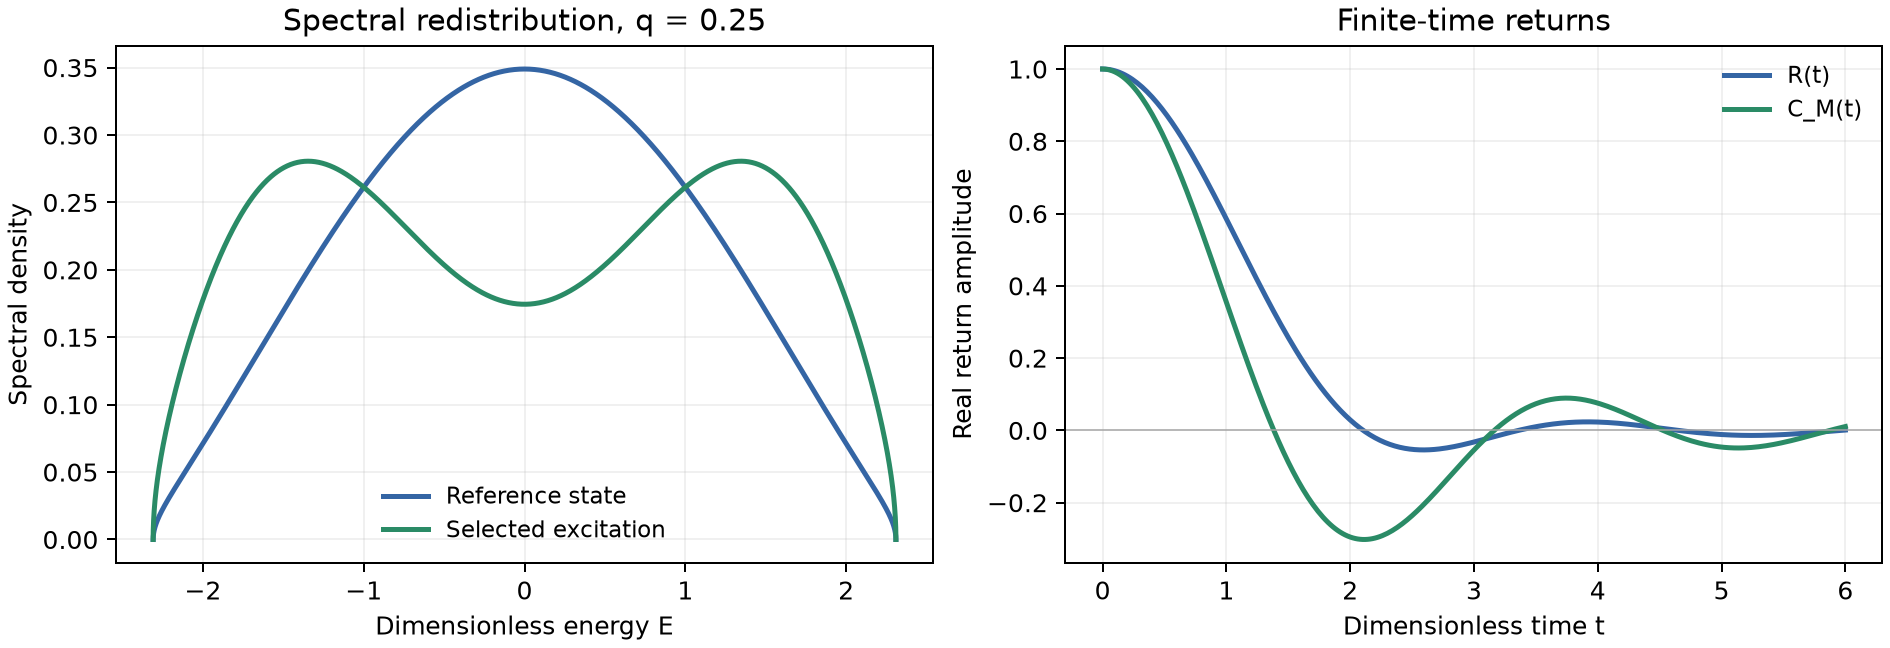
\includegraphics[width=\textwidth]{../../results/susskind-slater-transfer/selected-spectrum.png}
 \caption{Dimensionless $q=0.25$ spectral densities and return
 amplitudes from \eqref{selected}--\eqref{return}. The selected
 excitation redistributes weight toward larger $|E|$. The plotted
 times are fixed times in the limiting annealed representation.}
\end{figure}
The numerical calculation diagonalizes the real symmetric
$q$-Jacobi matrix at sizes 160 and 240, using its vacuum spectral
weights. It independently evaluates \eqref{density} with 256
product factors and 8,193 angular samples; normalization and
variance agree with one within $10^{-10}$. Fifteen selected
returns at three $q$ values agree between the two Jacobi sizes
to about $1.4\times10^{-15}$ or better.

For illustration, the filtered selected vector at $\beta=2$ has
the following energies in normalized $h$ units:
\begin{center}
\begin{tabular}{rrrr}
\toprule
$q$ & $Z_M(2)$ & $\langle h\rangle$ & $\operatorname{Var}(h)$\\
\midrule
0.0625 & 6.3522341 & -1.4597969 & 0.2546408\\
0.25   & 8.9789308 & -1.6651661 & 0.2437047\\
0.64   & 17.3664951 & -2.1157408 & 0.3337576\\
\bottomrule
\end{tabular}
\end{center}
These values describe Euclidean filtering, not a temperature
assigned to the full nonstationary state.

For an $L$-node Gaussian quadrature, polynomial exactness and
the compact support radius $E_* =2/\sqrt{1-q}$ give the
selected-return error bound in exact arithmetic
\begin{equation}
 2e^{|t|E_*}\frac{(|t|E_*)^{2L-2}}{(2L-2)!}.
\end{equation}
The degree-two selected weight explains the $2L-2$ exponent.
The saved numerical record separates this analytic truncation
bound from observed floating-point differences and imaginary
roundoff. It is not an interval certificate for the eigensolver.
At $t=0$ the saved logarithmic bound is $-\infty$, denoting
an exactly zero Taylor truncation bound.

\newpage
\section{Verification, preserved failure, and the next physics task}
The new transfer checker uses exact rational $\gamma=1/2,2/3$.
It compares 1,458 moments with the sealed sixth-word polynomials
and 232 eighth-word cases with independent pairing enumeration.
It additionally checks 248 algebra relations, 124 primitive
projection identities, 62 full tower decompositions, 680
adjunction entries, 170 metric symmetries and 54 residual-tower,
compression and selected-spectral identities. A separate checker
verifies 62 grading identities, 62 canonical commutators, 62
same-$J$ cross relations and 18 sharp selected-shift norms.

The initial checker failed before producing a scientific output:
Python integer division at the zero-level factorial introduced
a floating coefficient and a residual of about $8.7\times10^{-19}$.
The failed source and diagnosis are preserved. Changing that
coefficient to exact rational division resolved the failure;
the analytic decomposition was unchanged. Successful scientific
outputs were then sealed and not rerun. The three output records,
figure, parameters and environment versions are under
\texttt{results/susskind-slater-transfer/}; the evidence manifest
binds these to the document, two-pass build and page renders.

The transfer now supplies all joint correlators without explicit
pairing enumeration, while the primitive decomposition gives a
transparent Hamiltonian spectrum and selected preparation kernel.
The next target is to identify physically meaningful states and
observables in this explicit representation and compare their
propagation with the static-patch bulk requirements. In particular,
the grading reconstructed from $M$ needs a microscopic joint-sector
interpretation before it is called a spatial or radial observable.
Mass, locality, stationary observer conditions and finite-$G$
interactions remain tests to perform. Type I closure alone does
not establish that dictionary or a finite horizon entropy.

\begin{thebibliography}{9}
\bibitem{EP} E. G. Effros and M. Popa,
\emph{Feynman diagrams and Wick products associated with q-Fock space},
\href{https://arxiv.org/abs/math/0303045}{arXiv:math/0303045} (2003),
Secs.~2--3.
\bibitem{RX} H. Rajgadia and J. Xu,
\emph{Emergent States and Algebras from the Double-Scaling limit of
Pure States in SYK},
\href{https://arxiv.org/abs/2604.14387v3}{arXiv:2604.14387v3} (2026).
\bibitem{BNR} M. Berkooz, V. Narovlansky and H. Raj,
\emph{Complex Sachdev-Ye-Kitaev model in the double scaling limit},
\href{https://arxiv.org/abs/2006.13983v2}{arXiv:2006.13983v2} (2020),
Sec.~5.1.
\end{thebibliography}
\end{document}
